%\section{Run Directories \label{subchap:rundir}}

\section{Making a Run Directory}
Running RAM-SCB occurs not in the installation directory, but through \textit{run directories} -- special directories that keep your simulations separate from the installation and other simulations. To create a run directory, simply use the {\tt make} interface:
\begin{verbatim}
make rundir
\end{verbatim}
\noindent
{\tt make} will unpack some default inputs and organize a new directory aptly named {\tt run}. Note that if a run directory exists that is called ``run'', RAM-SCB will not over write it and {\tt make} will complain. 

Run directories soft link to the installation directory, so as long as you don't move, uninstall, or otherwise break your installation, you can put the run directory where ever you want. Furthermore, you are not limited to a single run directory. Adding more allows you to run more simulations simultaneously from a single installation. Using the {\tt PARAM} interface, described below, you can perform many very different simulations at once without re-compiling the code. The name and location of the run directory can be set using the RUNDIR variable as follows:
\begin{verbatim}
make rundir RUNDIR=/location/to/new/rundir
\end{verbatim}
\noindent

If running on a HPC cluster (or some other system with designated run spaces) it is important to place the run directories in the correct location. This can be done using the RUNDIR variable as above, or by moving the directory after to has been created:
\begin{verbatim}
make rundir
mv run /location/to/new/rundir
\end{verbatim}
\noindent

Both of the above methods produce the same result.

\section{Inside a Run Directory}
Let's look inside a typical run directory:

\begin{figure}[h]
 \begin{center}
  \includegraphics[width=25pc,clip=True,angle=90]{rundir.ps}
 \end{center}
 \caption{Run directory layout. Gray and green rounded boxes indicate subdirectories; green boxes are directories that are soft linked one level up for convenience. Yellow boxes are key input files, the red box is the linked RAM-SCB executable, and other data input files are listed without boxes.}
 \label{fig:rundir}
\end{figure}

Figure \ref{fig:rundir} shows the default run directory organization. The IM directory is where most input and output occurs; subdirectories shaded green are soft-linked to the top run level for convenience. These directories are self explanatory outside of {\tt output\_swmf}, which is for runs that use SWMF output in stand-alone mode. Enough inputs are given in the input directories for a sample simulation right away. The red box in Figure \ref{fig:rundir} denotes the linked executable. The final files, denoted as yellow boxes, are the final input files. {\tt w2k.dat} is the Weimer 2000 empirical model data file, {\tt omni.txt} is solar wind input file from the OMNI database, and {\tt RamIndices.txt} is a list of geomagnetic indices. The necessity of these three files is discussed below.

Finally, there is {\tt PARAM.in}, the run-time configuration file that is used to tell RAM-SCB what and how it should simulate. The {\tt PARAM} interface, identical to the one used by the SWMF, is simple. Any line of text in the file not preceeded by a \# symbol is ignored, so comment your file to your heart's content. Any text preceeded by \#, however, is a interpreted as a {\tt PARAM} command. A generic command takes the form,

\begin{verbatim}
#COMMANDNAME
Parameter1    ParameterName
Parameter2    ParameterName
...
ParameterN    ParameterName
\end{verbatim}

The exact values of the parameters are command specific; the parameter names are simply tab-delimited from the parameters and are not needed (keeping them is recommended to keep your file clear and easily understood!) Here are a few commands in action:

\begin{verbatim}
#STARTTIME 
2006	iYear 
7	iMonth 
19	iDay 
0	iHour 
0	iMinute 
0	iSecond

#OUTERBOUNDARY 
LANL	NameBoundPlasma 
T89C	NameBoundMag

#VARIABLEDT
T    DoVariableDt

#STOP
-1   MaxIteration
300   tSimulationMax
\end{verbatim}

First, take note that the parameter values can take many forms: rational numbers, integers, logical values, or strings of text. Remember that the trailing descriptions are not read by RAM-SCB; they are there to help you remember what each value does. In order, this list of {\tt PARAM} commands sets the start date and time of the simulation, sets the plasma and magnetic field outer boundary conditions, turns on variable timestepping, and tells the code to run for unlimited iterations but only 300 seconds. All commands are described in detail in Chapter \ref{chp:param}.

Once your {\tt PARAM} file is customized, execute RAM-SCB.

\begin{verbatim}
./ram_scb.exe
\end{verbatim}

RAM-SCB will begin; a lot of information will be written to screen that updates the user of its progress. Experienced Unix users know all of the tricks to capture that output; the following copies the output to file while preserving the output to screen:

\begin{verbatim}
./ram_scb.exe | tee runlog.txt
\end{verbatim}


\section{Required Inputs \label{subchap:input}}

Ring current models have three basic requirements: plasma fluxes at the outer boundary, magnetic field, and electric field throughout the equatorial plane. RAM-SCB fulfills these requirements slightly differently than other ring current models thanks to its sophisticated self-consistent magnetic field. Electric field may be specified either in the equatorial plane directly or as an ionospheric potential that is mapped along SCB field lines. Magnetic field is supplied as a shell surrounding the SCB domain, which consists of the body containing all field lines passing through the RAM equatorial domain. Plasma fluxes remain a simple specification about the outer boundary of RAM. In RAM-SCB, there are many ways to specify these; refer to Chapter \ref{chp:param} for commands that select inputs.

Plasma fluxes can be provided one of two ways: the first is coupling with the SWMF, covered in Chapter \ref{chp:swmf}. The second is to use ``GeoMlt'' files, a product of LANL geosynchronous observations. These files can be obtained on request from the data caretakers; sample files are provided with the distribution. These files come in pairs per day; an ion and electron file exists for each day for which there is data coverage. Because the source observations do not readily differentiate between different ion species, the $K_{P}$/$F_{10.7}$ dependent empirical relationship of \textit{Young et al.,} [1982] is used internally to divide up the Hydrogen flux in the input files. The $K_{P}$ and $F_{10.7}$ indices are packaged in the RamIndices.txt input file; the user need not worry about them for historical simulations.

Convection electric potential can be specified in a plethora of ways. The simplest is to use the $K_{P}$ dependent Volland-Stern electric field. This requires no additional input files beyond RamIndices.txt. The Weimer 2000 empirical model can also be used; like Volland-Stern, it is an internal calculation. Because this model depends on solar wind conditions, users must supply an input file that contains this data from the OMNI database. The Weimer 2000 potential is mapped along SCB field lines to the equatorial plane automatically. Finally, SWMF electric fields can be used; this is covered later. Though it is possible to supply Weimer 2000 and SWMF potentials in the equatorial plane without SCB mapping, this approach requires extensive work by the user as is not recommended. See the entry on the command \verb*l#EFIELDl for additional details on file formats and obtaining these inputs.

Magnetic field boundary conditions can be supplied via three sources: a simple dipole model, from one of the Tsyganenko empirical models, or from the SWMF. When using a dipole, it is possible to use a dipole with or without the SCB calculation. Tsyganenko 89 (T89) input files are provided with the distribution and require no additional input from the user. Input from more complex Tsyganenko models require substantial work to acquire, they are not recommended for most users. See the entry for the \verb*l#OUTERBOUNDARYl command in Chapter \ref{chp:param} for more details.

All files listed above must be placed in their respective input files in the run directory. Other input files required by advanced options (e.g. virtual satellites) should be placed in the top level of the run directory. Each run directory requires its own set of inputs.

\section{Restarting Simulations \label{subchap:restart}}
It is often desirable to split a simulation up into several parts. For example, you may want to split a very long simulation up into separate executions, or change parameters at certain parts of a storm, or perhaps a simulation was interrupted undesireably. Restart files allow you to continue a simulation seamlessly.

Throughout a simulation, restart files are being written to the {\tt restartOUT} folder of the run directory. The files are written at a set frequency and at the end of a successful run (both of these options are configuarble through the {\tt PARAM} interface.) Only the most recent restart is saved, users can periodically pull these files out of {\tt restartOUT} if they prefer a back log of restarts. These files contain the full distribution functions as well as the start time, current time, and current iteration at the point that the restart was written.

To restart a run, first move restart files from {\tt restartOUT} to {\tt restartIN}. Then, either create a new {\tt PARAM.in} file or edit the existing one such that no \verb*l#STARTTIMEl command is present (remember, the restart file knows this information already), the run time exceeds the current time listed in the restart file, and the command \verb*l#RESTARTl is included. This tells RAM-SCB to restart the simulation rather than start anew. Restarts are carefully implemented to preserve files in the output directories and continue the simulation as if there was no interruption.

For an example of restarting a simulation, run Test 2 and inspect the {\tt PARAM.in} files as well as the contents of {\tt restartIN} and {\tt restartOUT}.

\section{Output}
RAM-SCB, by default, has a rich output set. This can be expanded by activating other output file types via the {\tt PARAM} interface, be sure to review the commands listed in Chapter \ref{chp:param}. Table \ref{tab:out} summarizes the output that can be generated by RAM-SCB. Visualization of these files is covered in Chapter \ref{chp:viz}.


\begin{table}[ht]
 \centering
 \begin{tabular}{l l l l l}
 \hline\hline
  Type & Extension & Format & Default? & Contents\\
 \hline
 Log file & \verb*q*.logq & ASCII & Yes & Dst, integrated values\\
 Pressure files & \verb*l*.datl & ASCII & Yes & $\perp$ and $\parallel$ partial pressures\\
 E-Field files & \verb*l*.inl & ASCII & No & Equatorial electric potential\\
 Boundary files & \verb*l*.datl & ASCII & No & Fluxes at the outer boundary\\
 RAM flux files & \verb*l*.ncl & NetCDF & Yes & Full equatorial flux information\\
 Virtual Satellites &\verb*l*.ncl & NetCDF & No & Satellite specific values\\
 Field integral files &\verb*l*.datl & ASCII & Yes & $h$, $I$ geometric integrals\\
 Magnetic field file &\verb*l*.datl & ASCII & No & Full 3D SCB field\\
 Potential file &\verb*l*.datl & ASCII & No & Ionospheric electric potential\\
 3D pressure file&\verb*l*.datl & ASCII & No & Full 3D anisotropic pressure\\ 
 \end{tabular}
\caption{List of available output files.}
\label{tab:out}
\end{table}

